
\section{转换数据流图与控制流图到随机Petri网的方法} \label{sec:convert}

\subsection{本章使用的样例代码} \label{sec:codeeg}

\begin{figure}[!hbt]
\centering
    \lstinputlisting{code/func.cc}
\caption{本节使用的样例代码(以后简称代码E)} \label{fig:eg:code}
\end{figure}

本章使用如图 \ref{fig:eg:code} 所示的代码(以后简称代码E),来具体描述如何将数据流图、控制流图转换成为随机Petri网。
并在最终给出整合了数据流、控制流的随机Petri网,用以表示代码中的数据依赖。

这份代码结构简单明了,有循环结构、if单分支结构、switch多分支结构等,且包含常见的简单计算。
这些元素基本代表了所有的代码类型。







\subsection{转换控制流图到随机Petri网的方法}

\newsavebox{\egcfg}
\sbox{\egcfg}{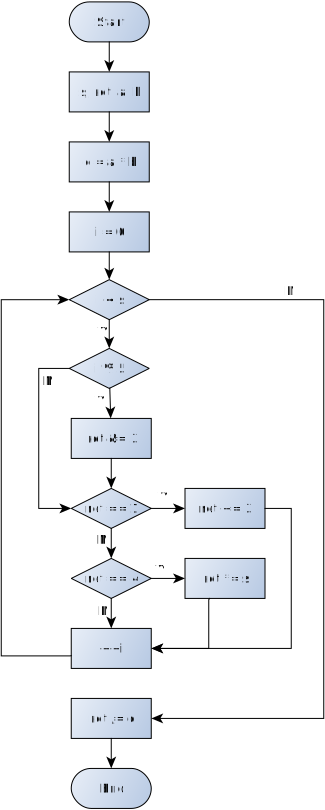
\includegraphics[totalheight=23cm]{image/eg-cfg.pdf}}
\begin{figure}[!hbt]
\centering
\usebox{\egcfg}
\caption{代码E的控制流图} \label{fig:eg:cfg}
\end{figure}

图 \ref{fig:eg:cfg} 给出了代码E的控制流图,并标明了每一个节点代表的操作。

\begin{algorithm}[!hbt]
\caption{将程序控制流图转换为随机Petri网} \label{alg:eg:cfg}
\begin{algorithmic}[1] %每行显示行号
  \Require $CFGEdge$ 控制流图中边的列表,$CFGNode$ 控制流图中节点列表
  \Ensure $PNEdge$ 随机Petri网中有向弧列表,$PNNode$ 随机Petri网中节点列表
    \Function{FillNodes}{$PNEdge, PNNode$}
      \For{$e=PNEdge.begin \to PNEdge.end$}
        \If{$e.head.type=e.tail.type$}
          \If{$e.head.type=Place$}
            \State $newNode \gets Trans("<nop>")$
          \Else
            \State $newNode \gets Place("")$
          \EndIf
          \State $newEdge.head \gets e.head$
          \State $newEdge.tail \gets newNode$
          \State $newEdge2.head \gets newNode$
          \State $newEdge2.tail \gets e.tail$
          \If{$newEdge.tail=Trans$}
            \State $newEdge.type = e.type$
          \Else
            \State $newEdge2.type = e.type$
          \EndIf
          \State $PNEdge.addedges(newEdge, newEdge2)$
          \State $PNEdge.remove(e)$
        \EndIf
      \EndFor
    \EndFunction

    \Function{GeneratePNet}{$CFGEdge, CFGNode$}
      \For{$n=CFGNode.begin \to CFGNode.end$}
        \If{$n.type=Branch$}
          \State $pnn \gets Place(n)$
        \Else
          \State $pnn \gets Trans(n)$
        \EndIf
        \State $PNNode.add(pnn)$
      \EndFor
      \For{$e=CFGEdge.begin \to CFGEdge.end$}
        \State $PNEdge.add(e.type)$
      \EndFor
      \State \Call{FillNodes}{$PNEdge, PNNode$}
      \State \Return $PNEdge, PNNode$
    \EndFunction
\end{algorithmic}
\end{algorithm}

对这个控制流图执行算法 \ref{alg:eg:cfg},可生成对应的随机Petri网。

算法 \ref{alg:eg:cfg} 首先这样定义输入数据:
将所有不会影响程序流程,即不会导致程序出现分支的运算,全部视为随机Petri网中的迁移。
将所有会影响程序流程,即所有会产生分支的运算,全部视为随机Petri网中的库所。
这样做的原因是:库所总会进入下一个迁移,而迁移可以是多个。
程序中分支控制的作用就是让程序进入不同的处理环节,各个处理环节对应着随机Petri网中的迁移。

对于每个分支,它们向迁移移动时都是矛盾的。
因此,算法 \ref{alg:eg:cfg} 根据控制图各边的属性,将回答为True的条件判断定义为默认的有向弧,将回答为False的条件判断定义为抑制弧。

对连续出现的判断做这样的处理:因为两个库所之间不应该有连线,所以在这样的两个库所之间添加一个空的迁移。
本文中对于这样的迁移,使用记号“<nop>”表示,即 Non-Operation。

对连续出现的迁移做这样的处理:因为两个迁移之间不应该有连线,所以在这样的两个迁移之间添加一个空的库所。

添加空的节点时,必须注意原来的有向弧的类型。做到连接到迁移上的有向弧类型要与原来的有向弧一致。

生成的对应的随机Petri网如图 \ref{fig:eg:cfgp} 所示。

\newsavebox{\egcfgp}
\sbox{\egcfgp}{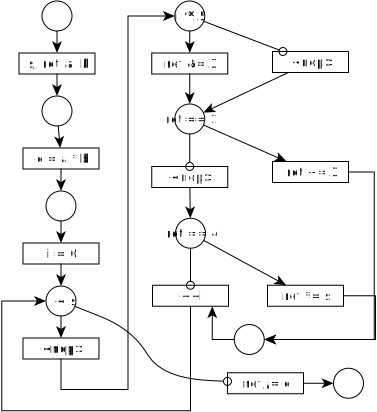
\includegraphics[totalheight=12cm]{image/eg-cfg-pnet.pdf}}
\begin{figure}[!hbt]
\centering
\usebox{\egcfgp}
\caption{代码E控制流图对应的随机Petri网} \label{fig:eg:cfgp}
\end{figure}





\subsection{转换数据流图到随机Petri网的方法}

下面介绍代码E的数据流图。

\subsubsection{不含控制信息的直接转换法}
如果无视控制流,数据流图经过简化后会显得非常小。没有控制信息的数据流图只能表示数据之间的依赖关系,而不能表示数据的真实流动。
图 \ref{alg:eg:dfg} 就是这样的一张图。它显得非常简短,信息量也非常少。因此只能用来查看大致的依赖情况,而不能真正用于分析程序的数据走向。

\newsavebox{\egdfg}
\sbox{\egdfg}{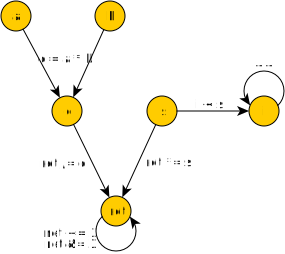
\includegraphics[totalheight=6cm]{image/eg-dfg.pdf}}
\begin{figure}[!hbt]
\centering
\usebox{\egdfg}
\caption{代码E不含控制流信息的数据依赖图} \label{fig:eg:dfg}
\end{figure}

对这样的图进行转换比较简单,算法 \ref{alg:eg:dfg} 进行了这样的转换。

\begin{algorithm}[!hbt]
\caption{将简化的数据依赖图转换为随机Petri网} \label{alg:eg:dfg}
\begin{algorithmic}[1] %每行显示行号
  \Require $DFGEdge$ 数据流图中边的列表,$DFGNode$ 数据流图中节点列表
  \Ensure $PNEdge$ 随机Petri网中有向弧列表,$PNNode$ 随机Petri网中节点列表
    \Function{GeneratePNet}{$DFGEdge, DFGNode$}
      \For{$n=DFGNode.begin \to DFGNode.end$}
        \If{$n.hasIngoing$}
          \State $p \gets PNNode.add(Place(n))$
          \State $t \gets PNNode.add(Trans)$
          \State $PNEdge.add(t, p)$
          \For{$i=n.ingoing.begin \to n.ingoing.end$}
            \State $p \gets PNNode.add(Place(i.head))$
            \State $PNEdge.add(p, t)$
          \EndFor
        \EndIf
      \EndFor
      \State \Return $PNEdge, PNNode$
    \EndFunction
\end{algorithmic}
\end{algorithm}

算法 \ref{alg:eg:dfg} 的行为很简单:将所有数据节点看成是库所,将所有入边合并为一个迁移。
这样数据依赖图就直接转化为随机Petri网,如图 \ref{fig:eg:dfgraw} 所示。

\newsavebox{\egdfgraw}
\sbox{\egdfgraw}{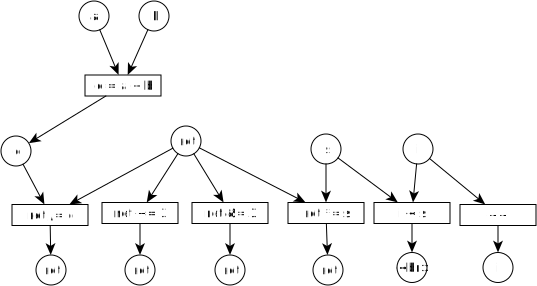
\includegraphics[totalheight=6cm]{image/eg-dfg-pnet.pdf}}
\begin{figure}[!hbt]
\centering
\usebox{\egdfgraw}
\caption{代码E不含控制流信息的数据依赖所对应的随机Petri网} \label{fig:eg:dfgraw}
\end{figure}

可以看到,图 \ref{fig:eg:dfgraw} 所示的随机Petri网虽然给出了各个数据的关系,
但它没能显示出每个数据自己的变化过程。而什么时候的数据依赖什么时候的数据,也没能显示出来。

这样的图丢失了时间关系和控制流程这些非常重要的信息,所以并不能够用于数据依赖的分析。
控制流和数据流是一个程序最基本的要素,要进行代码分析,二者缺一不可。

\subsubsection{引入控制流程的综合转换方法} \label{sec:dcfgconv}

这一节将控制流引入数据流的分析中。其方法是:以数据流分析为主,以控制流分析为辅。
分析得到的流程图应当与原程序契合,确保分析后得到的图形即是分析程序本身。

首先要得到包含控制信息的数据流程图。基本方法就是分析每一条指令,确认它对数据流向的影响。
又要注意分支对数据的影响。在图形的语义上要加以区分。

\newsavebox{\egdfgctrl}
\sbox{\egdfgctrl}{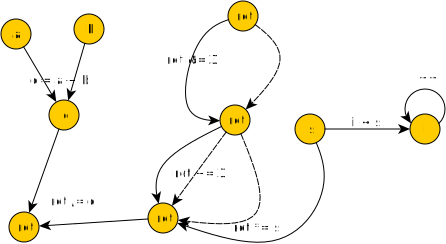
\includegraphics[width=12cm]{image/eg-dcfg.pdf}}
\begin{figure}[!hbt]
\centering
\usebox{\egdfgctrl}
\caption{代码E含控制流信息的数据流图} \label{fig:eg:dfgctrl}
\end{figure}

图 \ref{fig:eg:dfgctrl} 给出了对代码E进行上述分析后所得到的包含控制信息的数据流图。
图中使用实线表示一般情况下与条件判断为True时数据的走向,虚线表示条件判断为False时数据的走向。

通过这张图可以很明确地得知数据在程序中的变化情况,以及各阶段、各条件下数据之间相互依赖的关系。
但是,这张图有一个缺点,它丢失了分支的来源信息。例如图中s → ret这条线,应当与哪条线合并,单从图中是无法判断的。
所以,这张图因为丢失了关键信息,它本身是无法转化为随机Petri网的。

要解决这样的问题,首先是要找到包含分支流程等关键信息的结构。因为数据流图中不存在这些信息,所以要回溯到它的源头。
直接通过解析源代码来生成数据与控制流图,进而转换为相应的随机Petri网图,要比解析数据流图更加方便。
源码中含有程序的所有信息,将这些信息筛选整合为我们需要的信息即可。

当然,直接使用源代码是不可取的。C/C++语言语法复杂,自己编写分析器是十分困难的事情。
所以,这里借助LLVM这个已经非常成熟的工业级工具,帮助我们跳过C/C++语言的分析阶段,
从而可以直接分析结构整齐,同时又与源代码语义相同的bitcode。

基于LLVM所设计的数据与控制流分析算法如算法 \ref{alg:eg:dfgllvm} 所示。

\begin{algorithm}[!hbt]
\caption{基于LLVM的数据流——随机Petri网的转换} \label{alg:eg:dfgllvm}
\begin{algorithmic}[1] %每行显示行号
  \Require $FuncStruct$ LLVM架构中描述函数的结构
  \Ensure $EdgeList$ 随机Petri网中有向弧列表,$VarList$ 随机Petri网中节点列表
    \Function{Analyze}{$FuncStruct$}
      \For{$BB=FuncStruct.begin \to FuncStruct.end$} 
        \For{$II=BB.begin \to BB.end$}
          \If{$II.is(MemoryInst)$}
            \If{$VarList.find(II.target)$} 
              \State // 历史变量不会重新启用,只需分析新的寄存器
              \State $VarList.merge(II.target)$
            \Else
              \State $VarList.create(II.target)$
            \EndIf
          \ElsIf{$II.is(BinaryInst)$}
            \State // 数据的变换要继承当前基本块的属性
            \State $EdgeList.add(II.target, II.operand(0), BBList.getType(BB))$
            \State $EdgeList.add(II.target, II.operand(1), BBList.getType(BB))$
            \State // 设置变量位置,用于区分同名变量的不同状态
            \State $EdgeList.last.SetOrder(CurrentLoopIndex)$
          \ElsIf{$II.is(BranchInst)$}
            \State // 标记要视为抑制弧尾部的基本块
            \State $BBList.add(II.default, Common)$
            \State $BBList.add(II.inhibit, Inhibit)$
          \ElsIf{$II.is(SwitchInst)$}
            \State $BBList.add(II.default, Common)$
            \State $inhbrList \gets II.branchList$
            \For{$b=inhbrList.begin \to inhbrList.end$}
              \State $BBList.add(b, Inhibit)$
            \EndFor
          \EndIf
        \EndFor
      \EndFor
      \State $VarList.renameAll()$
      \State \Return $EdgeList, VarList$
    \EndFunction
    \Function{runOnFunction}{$FuncStruct$}
      \State \Return \Call{Analyze}{$FuncStruct$}
    \EndFunction
\end{algorithmic}
\end{algorithm}

这个算法虽然较为复杂,但因为是基于LLVM平台编写,输入对象是结构整齐的LLVM自定义图结构,因此有大量API帮助解析。
算法的详细过程:当opt程序在自行遍历图结构时,如果遇到函数结构,就会触发runOnFunction,从而触发这个解析算法。
算法将继续遍历这个函数子图,函数子图分为许多基本块(Basic Block,即算法中的迭代器BB),
基本块由许多指令(Instruction,即算法中的迭代器II)组成。算法根据指令的类型,执行相应的处理代码。

指令分为四大类:内存操作、二元计算、分支、switch分支。下面分别介绍针对这几类指令的处理方案:

{
\setstretch{1.0}
\begin{itemize}
    \addtolength{\itemindent}{2.5em}
    \item 内存操作分为创建虚拟寄存器(寄存器的命名同步进行)、读取数据、保存数据。
    \item 二元计算会将两个虚拟寄存器的结果进行二元计算,存到另一个虚拟寄存器中。
    \item 分支特指单分支。if、for、while都会生成单分支。
    \item switch分支也属于分支,但它较为特殊。它包含一个分支列表,算法必须解析这个列表,并如同处理单分支一样处理每个分支。
\end{itemize}
}

对于内存操作,算法要分析等价的变量(寄存器)。因为算法的输入是LLVM自定义的图结构,这样的结构,内部的指针与真实机器相差很远。
每个指针的指向不会改变,这对变量的等价分析很有帮助。等价分析会建立同义词表,同义词表的结果如同这样:如果变量A被读取,并被保存在了虚拟寄存器16中,
那么可以看作是,寄存器16与变量A等价,它们是同一个变量。另外,LLVM假定寄存器是无穷的,它会为每个操作分配一个新的寄存器号。
这样的行为会让每个变量在时间和空间上都是独立的。历史的变量永远成为历史,不会在未来重新启用,这可以保证变量的分析不会有冲突。

对于二元计算,算法要完成的任务是变量匹配。如果虚拟寄存器25要使用寄存器12和寄存器17相乘的结果,那么算法就会把12号、17号寄存器视作25号寄存器的依赖。

对于分支计算,算法要记住分支的来源,即它的判断曾经是True还是False,并做好相应的标记。
分支在LLVM语言里会表现为代码区块。对这样的区块内每一个指令都要加上和区块相同的标记,以便之后转换为普通有向弧或抑制弧。
LLVM的分支排列顺序是良好的,能够做到在遍历其中一个基本块时不漏下任何分支,因此不会漏下抑制弧的标记。

完成函数的遍历后要做收尾操作。算法要整理之前建立起来的同义词表,将等价的变量合并在一起并命名,从而生成最终的数据流图。
图的边和节点都会带有各自的属性,如一个有向弧是否是抑制弧等。这些属性组成了一个随机Petri网,代表了程序的数据与控制的流向。

经过算法 \ref{alg:eg:dfgllvm} 处理后的随机Petri网图会如同图 \ref{fig:eg:dfgctrlpnet} 所示。

\newsavebox{\egdfgctrlpnet}
\sbox{\egdfgctrlpnet}{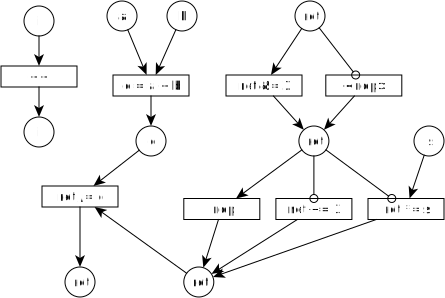
\includegraphics[width=11cm]{image/eg-dcfg-pnet.pdf}}
\begin{figure}[!hbt]
\centering
\usebox{\egdfgctrlpnet}
\caption{代码E含控制流信息的数据流图的随机Petri网} \label{fig:eg:dfgctrlpnet}
\end{figure}

这样的图可以非常直观地看出各个数据之间的流向、数据受到控制语句的影响、控制流的走向。
这个图包含了非常重要的时间与空间的信息,包含了控制与数据两类核心信息,同时还包含了二者之间紧密的联系。
这为分析程序的行为,分析程序的并行化重构的可能性提供了重要的依据。

补充:为了更直观地展现算法 \ref{alg:eg:dfgllvm} 的结构,图 \ref{fig:eg:dfgalgo} 简单地表示了这个算法的总体逻辑。

\newsavebox{\egdfgalgo}
\sbox{\egdfgalgo}{\includegraphics[totalheight=18.2cm]{image/core-algo.pdf}}
\begin{figure}[!hbt]
\centering
\usebox{\egdfgalgo}
\caption{数据流——随机Petri网转换算法的简单逻辑表示} \label{fig:eg:dfgalgo}
\end{figure}
